\section{Derivation \label{sec:derivation}}
This section is organized as follows, we will first derive a very basic sensing matrix\footnote{Here, we define the sensing matrix to be a matrix that maps sensor readouts to the displacements that we want to measure.}, assuming there's no misalignment in the optical system.
And then, we will derive the general sensing matrix that includes all sorts of misalignment.
Lastly, we will modify the matrix for a folded optical lever configuration.

In Sec.~\ref{sec:very_basic_derivation}, we will first derive the optical lever beam displacement due to a rotate and longitudinal shift of the sensing surface. 
In Sec.~\ref{sec:optical_levers_in_kagra}, we will derive the optical lever sensing matrix with a tilted plane of incidence, and reduce it to a horizontal and vertical configuration.
In Sec.~\ref{sec:misalignment}, we discuss some cross-coupling mechanism due to misalignment and correct the sensing matrice accordingly.
We also briefly touched on the folded optical lever configuration and discussed a cross-coupling mechanism exclusive to this setup, and provided a solution for this.
\subsection{Very basic derivation \label{sec:very_basic_derivation}}
\begin{figure}[!h]
	\centering
	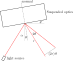
\includegraphics[width=73mm]{figures/optical_lever_rotation}
	\caption{A rotated reflective surface (the suspended optics) caused the optical lever beam to displace.}
	\label{fig:opticalleverrotation}
\end{figure}
In the simplest case, as shown in Fig.~\ref{fig:opticalleverrotation}, the beam position $x_1$ (along the incidence plane) is related to the angular displacement $\theta$ by
\begin{equation}
	x_1=\left(2r\right)\theta,
	\label{eqn:x1}
\end{equation}
where $r$ is the lever arm defined by the distance between the reflective surface and the sensing device.
The same beam can be used to measure the longitudinal displacement of the reflective surface, if the light beam has an angle of incidence $\alpha$, as shown in Fig.~\ref{fig:opticallevershifted}.
In this case, the beam displacement reads
\begin{equation}
	x_1=\left(2r\right)\theta + \left(2\sin{\alpha}\right)x_L,
	\label{eqn:beam_displacement_l}
\end{equation}
where $x_L$ is the longitudinal displacement of the reflective surface.
\begin{figure}[!h]
	\centering
	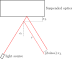
\includegraphics[width=72mm]{figures/optical_lever_shifted}
	\caption{A shift of the optical lever beam due to longitudinal shift of the reflective surface (the suspended optics).}
	\label{fig:opticallevershifted}
\end{figure}
As can be seen, equation.~\eqref{eqn:beam_displacement_l} shows a coupled sensor where it reads both the angular displacement and the longitudinal shift.

\begin{figure}[!h]
	\centering
	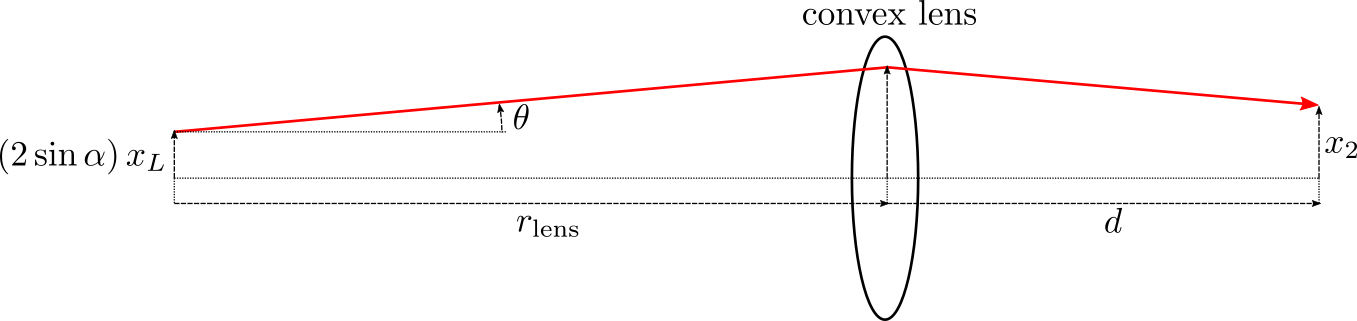
\includegraphics[width=134mm]{figures/optical_lever_lens}
	\caption{A second beam displacement sensor sensing the beam postion behind a lens.}
	\label{fig:opticalleverlens}
\end{figure}
In KAGRA, some optical levers have a second sensor measuring the beam displacement $x_2$ some distance $d$ behind a convex lens with focal length $f$, as shown in Fig.~\ref{fig:opticalleverlens}.
In this case, we obtain the second beam displacement $x_2$ via ray transfer matrices \cite{enwiki:1018856234}
\begin{equation}
	\begin{pmatrix}
		x_2\\
		\cdot
	\end{pmatrix}
	=
	\begin{bmatrix}
		1 & d\\
		0 & 1
	\end{bmatrix}
	\begin{bmatrix}
		1 & 0\\
		-1/f & 1
	\end{bmatrix}
	\begin{bmatrix}
		1 & r_\mathrm{lens} \\
		0 & 1
	\end{bmatrix}
	\begin{pmatrix}
		\left(2\sin{\alpha} \right)x_L\\
		2\theta
	\end{pmatrix},
\end{equation}
where $r_\mathrm{lens}$ is the distance between the reflective surface and the lens.
This gives
\begin{equation}
	x_2 = \left(2\sin\alpha\right)\left(1-\frac{d}{f}\right)x_L + 2\left[\left(1-\frac{d}{f}\right)r_\mathrm{lens}+d\right]\theta. 
	\label{eqn:beam_displacement_lens_1}
\end{equation}
Furthermore, we can place the second beam displacement sensor distance behind the lens.
So, if we set
\begin{equation}
	d=\frac{r_\mathrm{lens}f}{r_\mathrm{lens}-f},
	\label{eqn:d}
\end{equation}
then the angular coupling, i.e. the second term in Eqn.~\eqref{eqn:beam_displacement_lens_1}, becomes zero, effectively making the second beam displacement sensor a ``length'' (length as in longitudinal displacement) sensing device.
If Eqn.~\eqref{eqn:d} is satisfied, then the beam displacement measured by the second senor reads
\begin{equation}
	x_2 = \left(\frac{-2f\sin\alpha}{r_\mathrm{lens}-f}\right)x_L.
	\label{eqn:x2}
\end{equation}
Now, if we put Eqn.~\eqref{eqn:beam_displacement_l} and Eqn.~\eqref{eqn:x2} in a matrix form, we can obtain the sensing matrix, i.e.
\begin{equation}
	\begin{pmatrix}
		x_L\\
		\theta
	\end{pmatrix}
	=
	\begin{bmatrix}
		2\sin\alpha & 2r\\
		\frac{-2f\sin\alpha}{r_\mathrm{lens}-f} & 0
	\end{bmatrix}^{-1}
	\begin{pmatrix}
		x_1\\
		x_2
	\end{pmatrix}
\end{equation}
Then, from here, we can diagonalize\footnote{
Consider a model $\vec{y}=\mathbf{C}\vec{x}$, where $\vec{y}$ are the measurements, and $\vec{x}$ are the states.
The goal is to define another measurement basis $\vec{y'}$ such that $\vec{y'}=\mathbf{C'}\vec{x}$, where $\mathbf{C'}$ is a diagonal matrix.
It's obvious that If we define $\vec{y'}\equiv\mathbf{C}^{-1}\vec{y}$, then $\mathbf{C'}$ becomes the identity, which is a diagonal matrix.
Therefore, we define $\mathbf{C}^\mathrm{-1}$ to be the sensing matrix, which maps sensor measurements to the displacements of the reflective surface.
}
the sensors.

\subsection{Optical levers in KAGRA \label{sec:optical_levers_in_kagra}}
Before diving into the discussion of misalignment, let's rewrite the matrix so it's closer to what we see in KAGRA.

In KAGRA, we have two beam displacement sensors\footnote{Some only has one, e.g. MCo.}, tilt-sensing QPD and length-sensing QPD. They are analogous to the first and second beam position sensors in Sec.~\ref{sec:very_basic_derivation}, respectively.
Each QPD has two readouts, the horizontal and the vertical displacement of the beam spot, denoted ($x_\mathrm{tilt}$, $y_\mathrm{tilt}$), and ($x_\mathrm{len}$, $y_\mathrm{len}$) for tilt-sensing QPD and length-sensing QPD respectively.
Here, note that the displacements sensed by the QPDs are not, in general, parallel to the global horizontal or vertical plane, as the QPDs are virtually placed orthogonal to the beam.
We are particularly interested in the optics' longitudinal $x_L$, pitch $\theta_P$, and yaw $\theta_Y$ displacements.
Therefore, the goal is to find a matrix that maps $\vec{x}=\left(x_\mathrm{tilt},\, y_\mathrm{tilt},\, x_\mathrm{len},\, y_\mathrm{len}\right)^T$ to longitudinal displacement, pitch angle, and yaw angle $\left(x_L,\, \theta_P,\, \theta_Y\right)^T$.

\begin{figure}[!h]
	\centering
	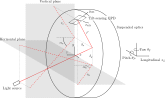
\includegraphics[width=0.7\linewidth]{figures/kagra_optical_lever_3d}
	\caption{Tilt-sensing optical lever setup in KAGRA.}
	\label{fig:kagraopticallever3d}
\end{figure}

A 3D illustration of the a general tilt-sensing optical lever setup is shown in Fig.~\ref{fig:kagraopticallever3d}.
For the current discussion, let's assume that the optical lever is well aligned so the beam spot miscentering at the optics $\delta_x$ and $\delta_y$ are zero.
Now, the lever arm of the optical lever can be an arbitrary vector, i.e. $\vec{r}=r_x\hat{x}+r_y\hat{y}+r_z\hat{z}$.
For the purpose of this discussion, let $\hat{x}$ be a direction aligned to the transverse direction of the main optics, $\hat{y}$ be a direction aligned to the vertical direction of the optics, and $\hat{z}$ be a direction aligned to the longitudinal direction of the optics.
Optical levers in KAGRA are aligned on a horizontal plane (i.e. $r_y=0$), or vertical plane (i.e. $r_x=0$).
But, let's assume that they are not zero.

If we project the beam onto a horizontal plane and a vertical plane (along the normal of the suspended optics), the beams have an incidence angle of $\alpha_h$ and $\alpha_v$ on the horizontal plane and the vertical plane, respectively.
It follows that the lever arm that amplifies the pitch angle is the length of the projection of the lever arm $\vec{r}$ on the vertical plane, $r_v$\footnote{Think of it as a cross-product $\vec{\theta}\times\vec{r}$. For example, for pitch, $-\theta_P\hat{x}\times\left(r_x\hat{x}+r_y\hat{y}+r_z\hat{z}\right) = \theta_P\left(-r_y\hat{z}+r_z\hat{y}\right)$, which is a displacement on the horizontal plane, and $r_v=\sqrt{r_y^2+r_z^2}$ is the corresponding lever arm that amplifies pitch.}.
Similarly, the lever arm amplifying the yaw angle is the length of the projection of the lever arm on the horizontal plane, $r_h$.
Therefore, a rotation in yaw $\theta_Y$ and pitch $\theta_P$ would cause the beam spot at the tip of the lever arm to shift by $\left(2r_h\right)\theta_Y$ and $\left(2r_v\right)\theta_P$, on the horizontal plane and vertical plane respectively.
Meanwhile, a longitudinal shift $x_L$ would cause the beam spot to shift by $\left(2\sin\alpha_h\right)x_L$ and $\left(2\sin\alpha_v\right)x_L$ on the horizontal plane and vertical plane, respectively.
From here, we can write the displacement of the beam spot as measured by the tilt-sensing QPD, placed at some distance $\vec{r}$ from the beam spot at the suspended optics plane.
The beam spot displacement is simply a superposition of that caused by a rotation and a longitudinal shift,
\begin{equation}
	x_\mathrm{tilt} = \left(2r_h\right)\theta_Y + \left(2\sin\alpha_h\right)x_L,
	\label{eqn:x_tilt}
\end{equation}
and
\begin{equation}
	y_\mathrm{tilt} = \left(2r_v\right)\theta_P + \left(2\sin\alpha_v\right)x_L.
	\label{eqn:y_tilt}
\end{equation}

As for the length-sensing QPD, let's assume that beam travels some displacement $\vec{r}_\mathrm{lens}$ from the suspended optics to a convex lens with focal length $f$. Fig.~\ref{fig:kagralengthopticallever3d} shows the length-sensing optical lever setup.
Here, note that the beam in Fig.~\ref{fig:kagralengthopticallever3d} is common to that in Fig.~\ref{fig:kagraopticallever3d}\footnote{In reality, there's a beamsplitter in front of the tilt-sensing QPD to divide the beam into two.}.
\begin{figure}[!h]
	\centering
	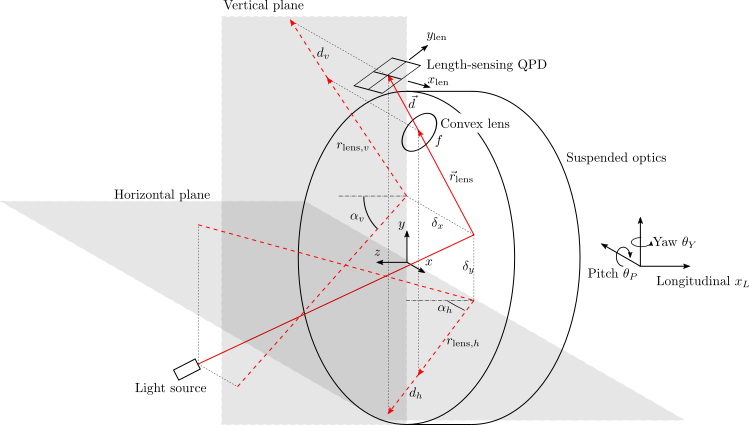
\includegraphics[width=0.7\linewidth]{figures/kagra_length_optical_lever_3d}
	\caption{Length-sensing optical lever setup in KAGRA.}
	\label{fig:kagralengthopticallever3d}
\end{figure}

Let's say the horizontal lever arm from the optics to the convex lens is $r_{\mathrm{lens},h}$.
Again, using ray transfer matrix, we can write down the  beam spot displacement at the length-sensing QPD,
\begin{equation}
	x_\mathrm{len} = \left(2\sin\alpha_h\right)\left(1-\frac{d_h}{f}\right)x_L + 2\left[\left(1-\frac{d_h}{f}\right)r_{\mathrm{lens},h},+d_h\right]\theta_Y,
	\label{eqn:x_len}
\end{equation}
where $d_h$ is the length between the lens and the length-sensing QPD on the horizontal plane, and $f$ is the focal length of the lens.
It follows that when $d_h=\frac{r_{\mathrm{lens},h}f}{r_{\mathrm{lens},h}-f}$, $x_\mathrm{len}$ is decoupled from yaw.
But, $d_h$ is a distance on the horizontal plane.
To get back the length, $d$, we can simply use a similar triangle relationship, as shown in Fig.~\ref{fig:dh},
\begin{equation}
	\begin{split}
	d_\mathrm{yaw} + r_\mathrm{lens} &= \left(d_h+r_{\mathrm{lens} h}\right)\frac{r_\mathrm{lens}}{r_{\mathrm{lens},h}},\\
	d_\mathrm{yaw} &= \left(d_h+r_{\mathrm{lens}, h}\right)\frac{r_\mathrm{lens}}{r_{\mathrm{lens},h}} - r_\mathrm{lens}\\
	\end{split}
\end{equation}
\begin{figure}[!h]
	\centering
	
\includegraphics[width=46mm]{figures/d_h}
	\caption{A similar triangle formed by the beam and it's projection on the horizontal plane (length-sensing QPD path).}
	\label{fig:dh}
\end{figure}
Here, if we set $d=d_\mathrm{yaw}$, then the horizontal readout of the length-sensing QPD $x_\mathrm{len}$ will have no yaw coupling, i.e.
\begin{equation}
	x_\mathrm{len} = \left(\frac{-2f\sin\alpha_h}{r_{\mathrm{lens},h}-f}\right)x_L.
\end{equation}
However, in this case, the vertical readout $y_\mathrm{len}$ is \textbf{not} decoupled from pitch, in general.
Now, if we set $d=d_\mathrm{yaw}$, then, on the vertical plane, $d_v$ reads, again, from similar triangle relation,
\begin{equation}
	\begin{split}
	d_v &= \left(d_\mathrm{yaw}+r_\mathrm{lens}\right)\frac{r_{\mathrm{lens},v}}{r_\mathrm{lens}} - r_{\mathrm{lens},v}\\
	&= \left(d_h+r_{\mathrm{lens},h}\right)\frac{r_{\mathrm{lens},v}}{r_{\mathrm{lens},h}}-r_{\mathrm{lens},v}\\
	&= \left(\frac{r_{\mathrm{lens},h}f}{r_{\mathrm{lens},h}-f}+r_{\mathrm{lens},h}\right)\frac{r_{\mathrm{lens},v}}{r_{\mathrm{lens},h}}-r_{\mathrm{lens},v}\\
	&=\left(\frac{r_{\mathrm{lens},h}}{r_{\mathrm{lens},h}-f}-1\right)r_{\mathrm{lens},v}\\
	&=\frac{r_{\mathrm{lens},v}f}{r_{\mathrm{lens},h}-f}
	\end{split}
\end{equation}
whereas if we want $y_\mathrm{len}$ to be decoupled from pitch, we need to set
\begin{equation}
	d_v = \frac{r_{\mathrm{lens},h}f}{r_{\mathrm{lens},h}-f},
\end{equation}
In general, $r_{\mathrm{lens},h}\neq r_{\mathrm{lens},v}$.
So, we cannot simultaneously decouple pitch and yaw from the length-sensing readout.
And, if we choose to set $d=d_\mathrm{yaw}$, i.e. to minimize yaw coupling, the vertical length-sensing QPD readout reads
\begin{equation}
	\begin{split}
	y_\mathrm{len} &= \left(2\sin\alpha_v\right)\left(1-\frac{d_v}{f}\right)x_L + 2\left[\left(1-\frac{d_v}{f}\right)r_{\mathrm{lens},v}+d_v\right]\theta_P\\
	&= \left(2\sin\alpha_v\right)\left(\frac{r_{\mathrm{lens},h}-r_{\mathrm{lens},v}-f}{r_{\mathrm{lens},h}-f}\right)x_L + 2\left[\left(\frac{r_{\mathrm{lens},h}-r_{\mathrm{lens},v}-f}{r_{\mathrm{lens},h}-f}\right)r_{\mathrm{lens},v} + \frac{r_{\mathrm{lens},v}f}{r_{\mathrm{lens},h}-f}\right] \theta_P\\
	&=\left(2\sin\alpha_v\right)\left(\frac{r_{\mathrm{lens},h}-r_{\mathrm{lens},v}-f}{r_{\mathrm{lens},h}-f}\right)x_L
	+ 2\left[\left(\frac{r_{\mathrm{lens},h}-r_{\mathrm{lens},v}}{r_{\mathrm{lens},h}-f}\right)r_{\mathrm{lens},v}\right] \theta_P.
	\end{split}
	\label{eqn:y_len}
\end{equation}
Here, note that if the length of the projections are equal, i.e. $r_{\mathrm{lens},h}=r_{\mathrm{lens},h}$, then vertical readout of the length-sensing QPD is decoupled from pitch.
This refers to a rather interesting configuration, where the incidence plane of the beam is rotated $45^\circ$ along the $z$-axis with respect to the vertical plane.

Without loss of generality, let's assume arbitrary\footnote{They can't be completely arbitrary. They must be related via the angle between the horizontal plane and the plane of incidence. But, I don't want to introduce that unnecessary parameter.} $d_h$ and $d_v$, and write the sensing matrix $\mathbf{C}_\mathrm{align}$ for a perfectly aligned optical lever.
If we ensemble Eqn.~\eqref{eqn:x_tilt}, \eqref{eqn:y_tilt}, \eqref{eqn:x_len}, and the first line of \eqref{eqn:y_len} into a matrix form, we get
\begin{equation}
	\begin{pmatrix}
		x_L\\
		\theta_P\\
		\theta_Y
	\end{pmatrix}
	=
	\mathbf{C}_\mathrm{align}
	\begin{pmatrix}
		x_\mathrm{tilt}\\
		y_\mathrm{tilt}\\
		x_\mathrm{len}\\
		y_\mathrm{len}
	\end{pmatrix},
	\label{eqn:sensing_matrix_general}
\end{equation}
where
\begin{equation}
	\mathbf{C}_\mathrm{align}
	=
	\begin{bmatrix}
		2\sin\alpha_h & 0 & 2r_h\\
		2\sin\alpha_v & 2r_v & 0\\
		2\sin\alpha_h\left(1-\frac{d_h}{f}\right) & 0 & 2\left[\left(1-\frac{d_h}{f}\right)r_{\mathrm{lens},h}+d_h\right]\\
		2\sin\alpha_v\left(1-\frac{d_v}{f}\right) &  2\left[\left(1-\frac{d_v}{f}\right)r_{\mathrm{lens},v}+d_v\right] & 0\\
	\end{bmatrix}^{+},
\end{equation}
Here, $\begin{bmatrix}\cdot\end{bmatrix}^{+}$ is the pseudoinverse of $\begin{bmatrix}\cdot\end{bmatrix}$, and $\begin{bmatrix}\cdot\end{bmatrix}^{+}\begin{bmatrix}\cdot\end{bmatrix}=\mathbf{I}$.

\subsubsection{Horizontal optical levers \label{sec:horizontal_optical_levers}}
Eqn.~\eqref{eqn:sensing_matrix_general} gives a general relationship between the QPD readouts and the displacements of the optics without misalignments.
It can be drastically simplified if we further assume that the incidence plane is aligned to the horizontal plane (e.g. Type-Bp and Type-A) or the vertical plane (e.g. Type-B). 
For horizontal optical levers, $\alpha_v=0$.
This gives $y_\mathrm{tilt}=\left(2r_v\right)\theta_P$ and $y_\mathrm{len}=2\left[\left(1-\frac{d_v}{f}\right)r_{\mathrm{lens},v}+d_v\right]\theta_P$, which are not independent from each other.
We can choose to omit the readout $y_\mathrm{len}$ and hence the sensing matrix for a horizontal optical lever is
\begin{equation}
	\begin{pmatrix}
		x_L\\
		\theta_P\\
		\theta_Y
	\end{pmatrix}
	=
	\begin{bmatrix}
		2\sin\alpha_h & 0 & 2r_h\\
		0 & 2r_v & 0\\
		\frac{-2f\sin\alpha_h}{r_{\mathrm{lens},h}-f} & 0 & 0
	\end{bmatrix}^{-1}
	\begin{pmatrix}
		x_\mathrm{tilt}\\
		y_\mathrm{tilt}\\
		x_\mathrm{len}
	\end{pmatrix},
	\label{eqn:sensing_matrix_horizontal}
\end{equation}
where we've assumed $d=d_h=\frac{r_{\mathrm{lens},h}f}{r_{\mathrm{lens},h}-f}$.
Note that on a horitonzal setup, the beam is on the horizontal plane so the horizontal lever arm $r_h=r$.
Furthermore, the projection on the vertical plane is simply $r_v=r\cos\alpha_h$.
Similarly, the horizontal arm displacement from the optics to the lens $r_{\mathrm{lens},h}=r_\mathrm{lens}$.

\subsubsection{Vertical optical levers}
Like in Sec.~\ref{sec:horizontal_optical_levers}, without further derivation, we can write the sensing matrix for a vertical optical lever setup.
\begin{equation}
	\begin{pmatrix}
		x_L\\
		\theta_P\\
		\theta_Y
	\end{pmatrix}
	=
	\begin{bmatrix}
		0 & 0 & 2r_h\\
		2\sin\alpha_v & 2r_v & 0\\
		\frac{-2f\sin\alpha_v}{r_{\mathrm{lens},v}-f} & 0 & 0
	\end{bmatrix}^{-1}
	\begin{pmatrix}
		x_\mathrm{tilt}\\
		y_\mathrm{tilt}\\
		y_\mathrm{len}
	\end{pmatrix},
	\label{eqn:sensing_matrix_vertical}
\end{equation}
where we've set $d=d_v=\frac{r_{\mathrm{lens},v}f}{r_{\mathrm{lens},v}-f}$.
Again, for a vertical setup, $r_v=r$, $r_h=r\cos\alpha_v$, and $r_{\mathrm{lens},v}=r_\mathrm{lens}$.

\subsubsection{Short summary}
We have derived the sensing matrix, Eqn.~\eqref{eqn:sensing_matrix_general}, assuming no misalignment, for a general optical lever setup with a tilted incidence plane.
From that, we reduced the general matrix to Eqn.~\eqref{eqn:sensing_matrix_horizontal} and \eqref{eqn:sensing_matrix_vertical}, which corresponds to the sensing matrix for a horizontal optical lever setup and vertical optical lever setup, respectively.
In general, the angle of incidence, arm lengths, and focal length are known.
Therefore, Eqn.~\eqref{eqn:sensing_matrix_horizontal} and \eqref{eqn:sensing_matrix_vertical} can be used as initial sensing matrices for the Type-Bp/Type-A and Type-B optical levers, respectively.


\subsection{Cross-coupling due to misalignment\label{sec:misalignment}}
Eqn.~\eqref{eqn:sensing_matrix_horizontal} and \eqref{eqn:sensing_matrix_vertical} give initial sensing matrices for converting the QPD readouts $\left(x_\mathrm{tilt},\,y_\mathrm{tilt},\,x_\mathrm{len},\,y_\mathrm{len}\right)$ to longitudinal $x_L$, pitch $\theta_P$, and yaw $\theta_Y$.
However they are ``initial'' sensing matrix only
There might still be residual cross-couplings between channels and the sensing matrices must be processed to minimize these couplings.
In this section, we will discuss 3 mechanisms due to misalignment of the optical lever that could lead to cross-coupling between the three displacements, namely, rotation of the QPD frame, miscentering of the QPD beam at the optics plane, and misplacement of the length-sensing QPD.
And, we will modify Eqn.~\eqref{eqn:sensing_matrix_general} accordingly.

\subsubsection{Rotated QPD frame}
There's no reason why the QPD is exactly aligned to the a desired frame in the first place.
In fact, the QPD frame can easily be rotated with respective to the desired frame.
There are many ways how this could happen.
For example, the QPD could be physically rotated.
Or maybe there's a steering mirror in the middle that caused this rotation.
Therefore, we must that this effect into account and make necessary corrections.

\begin{figure}[!h]
	\centering
	
\includegraphics[width=80mm]{figures/rotation}
	\caption{A rotational between the ``yaw-pitch'' frame (primed frame in red) and the tilt-sensing QPD frame (unprimed frame in black).}
	\label{fig:rotation}
\end{figure}
Take the tilt-sensing QPD for example.
Fig.~\ref{fig:rotation} shows a rotation between the ``yaw-pitch'' frame and the tilt-sensing QPD frame.
In the figure, red axes indicates the direction of the beam spot displacement when subjected to a pure yaw displacement and pure pitch displacement.
This means that, the primed horizontal displacement $x_\mathrm{tilt}'$ reads
\begin{equation}
	x_\mathrm{tilt}'=\left(2r_h\right)\theta_Y + \left(2\sin\alpha_h\right)x_L,
\end{equation}
and the primed vertical displacement reads
\begin{equation}
	y_\mathrm{tilt}'=\left(2r_v\right)\theta_P + \left(2\sin\alpha_v\right)x_L.
	\label{eqn:y_tilt'}
\end{equation}
These are the quantities that we should be reading.
But instead, we are reading the QPD readouts $x_\mathrm{tilt}$ and $y_\mathrm{tilt}$, which are not aligned with $x_\mathrm{tilt}'$ and $y_\mathrm{tilt}'$.

Here, the primed frame is a rotated by an angle $\phi_\mathrm{tilt}$ compared to the QPD frame.
Hence, we can relate the two frames via 
\begin{equation}
	\begin{bmatrix}
		\cos\phi_\mathrm{tilt} & \sin\phi_\mathrm{tilt}\\
		-\sin\phi_\mathrm{tilt} & \cos\phi_\mathrm{tilt}
	\end{bmatrix}
	\begin{pmatrix}
		x_\mathrm{tilt}\\
		y_\mathrm{tilt}
	\end{pmatrix}
	=
	\begin{pmatrix}
		x_\mathrm{tilt}'\\
		y_\mathrm{tilt}'
	\end{pmatrix}.
\end{equation}
A similar operation can be done to the length-sensing readout $x_\mathrm{len}$ and $y_\mathrm{len}$, but with a different angle $\phi_\mathrm{len}$.
So, Eqn.~\eqref{eqn:sensing_matrix_general} must be modified to
\begin{equation}
	\begin{pmatrix}
		x_L\\
		\theta_P\\
		\theta_Y
	\end{pmatrix}
	=
	\mathbf{C}_\mathrm{align}
	\mathbf{C}_\mathrm{rotation}
	\begin{pmatrix}
		x_\mathrm{tilt}\\
		y_\mathrm{tilt}\\
		x_\mathrm{len}\\
		y_\mathrm{len}
	\end{pmatrix},
	\label{eqn:sensing_matrix_general_rotation}
\end{equation}
where $\mathbf{C}_\mathrm{align}$ is the sensing matrix for the perfectly aligned optical lever, i.e. sensing matrix in Eqn.~\eqref{eqn:sensing_matrix_general},
and
\begin{equation}
	\mathbf{C}_\mathrm{rotation}
	=
	\begin{bmatrix}
		\cos\phi_\mathrm{tilt} & \sin\phi_\mathrm{tilt} & 0 & 0\\
		-\sin\phi_\mathrm{tilt} & \cos\phi_\mathrm{tilt} & 0 & 0\\
		0 & 0 & \cos\phi_\mathrm{len} & \sin\phi_\mathrm{len} \\
		0 & 0 & -\sin\phi_\mathrm{len} & \cos\phi_\mathrm{len}
	\end{bmatrix}
\end{equation}
is the matrix to correct rotated QPDs.

There's a caveat in this correction, that is, we assume the QPD axes are orthogonal.
While this is a very legitimate assumption, this may not be the case if the 4 photodiodes of the QPD has slightly different sensitivities.
In this case, we should rotate the axes separately with different angles.
However, we shouldn't allow such asymmetric rotation since the calibrations will not be preserved.
So, it's meaningless to include this kind of correction into the sensing matrix.
Instead, it should be corrected during the calibration stage, where the problem should have been discovered.
Or we can simply discover this by observing the fluctuation in QPD sum.
If the sensitivities don't match, then there will be large fluctuation in the QPD sum.

There's also an important note here.
The rotational transformation should be applied directly to the QPD beam spot displacements readout, not the calibrated yaw-pitch readouts.
This is as basic as knowing that matrices don't commute.
If to mix the order of matrix multiplication,
this can, of course, still decouple yaw and pitch.
But, it will completely mess up the calibration because pitch and yaw don't necessarily have the same lever arm coupling.

\subsubsection{Miscentered beam spot \label{sec:miscentered_beam_spot}}
Previous derivation assumes that the beam hits the optics at the center of rotation.
But, in general, the beam will be miscentered by some small amount $\delta_x$ and $\delta_y$ in the horizontal and vertical direction, respectively, as shown in Fig.~\ref{fig:kagraopticallever3d} and Fig.~\ref{fig:kagralengthopticallever3d}.
In this case, rotation-to-longitudinal cross-couplings will be introduced.

\begin{figure}[!h]
	\centering
	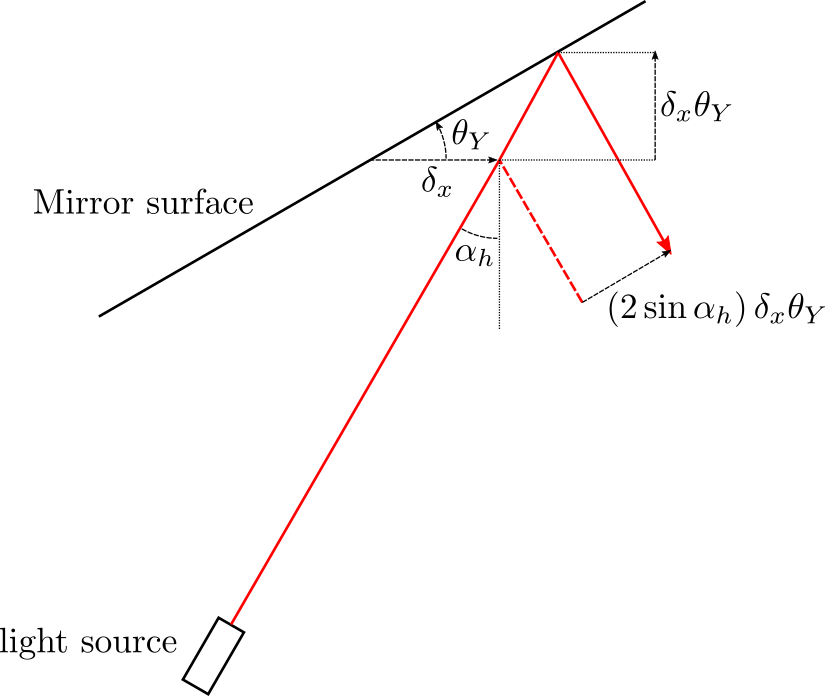
\includegraphics[width=80mm]{figures/miscentered}
	\caption{The beam spot of the optical lever beam at the optics plane is miscentered by an amount of $\delta_x$ horizontally with respect to the rotational axis. Note that the yaw angle $\theta_Y$ is largely exaggerated.}
	\label{fig:miscentered}
\end{figure}
Fig.~\ref{fig:miscentered} shows a horizontally miscentered optical lever beam.
In Eqn.~\eqref{eqn:beam_displacement_l}, the displacement $\left(2\sin\alpha\right)x_L$ is the shift of the beam from the original optical axis.
If the beam spot is off-centered, say by an amount of $\delta_x$ in the horizontal direction, a rotation in the yaw direction will also introduce a longitudinal shift of the beam spot at the optics plane by an amount of $\delta_x\theta_Y$. 
This correspond to a parallel beam shift by an amount of $\left(2\sin\alpha_h\right)\delta_x\theta_Y$\footnote{To the first order correction only. In reality, the angle of incidence is $\alpha_h+2\theta_Y$, but not $\alpha_h$. Here, we assume $\theta_Y$ is small, so $\sin\alpha_h \approx \sin{\left(\alpha_h+2\theta_Y\right)}$}.
Similarly, if the beam spot is off-centered in the vertical direction by an amount $\delta_y$, a rotation in the pitch direction will introduce a longitudinal shift of $\delta_y\theta_P$.
This correspond to a parallel beam shift by an amount of $\left(2\sin\alpha_v\right)\delta_y\theta_P$.

Note that the first row of Eqn.~\eqref{eqn:sensing_matrix_general} longitudinal shift of the optics $x_L$.
To correct for miscentered beam spot, we can simply replace $x_L$ by the longitudinal shift of the beam spot at the optics plane, i.e. $x_L + \delta_y\theta_P + \delta_x\theta_Y$.
This correspond to multiplying a matrix on the left-hand side of the equation, i.e.
\begin{equation}
	\begin{pmatrix}
		x_L+\delta_y\theta_P+\delta_x\theta_Y\\
		\theta_P\\
		\theta_Y
	\end{pmatrix}
	=
	\begin{bmatrix}
		1 & \delta_y & \delta_x\\
		0 & 1 & 0\\
		0 & 0 & 1
	\end{bmatrix}
	\begin{pmatrix}
		x_L\\
		\theta_P\\
		\theta_Y
	\end{pmatrix}.
\end{equation}
Therefore, to account for beam miscentering, Eqn.~\ref{eqn:sensing_matrix_general_rotation} must be further modified to
\begin{equation}
	\begin{pmatrix}
		x_L\\
		\theta_P\\
		\theta_Y
	\end{pmatrix}
	=
	\mathbf{C}_\mathrm{miscenter}
	\mathbf{C}_\mathrm{align}
	\mathbf{C}_\mathrm{rotation}
	\begin{pmatrix}
		x_\mathrm{tilt}\\
		y_\mathrm{tilt}\\
		x_\mathrm{len}\\
		y_\mathrm{len}
	\end{pmatrix},
	\label{eqn:sensing_matrix_general_misalignment}
\end{equation}
where
\begin{equation}
	\mathbf{C}_\mathrm{miscenter}
	=
	\begin{bmatrix}
		1 & \delta_y & \delta_x\\
		0 & 1 & 0\\
		0 & 0 & 1
	\end{bmatrix}^{-1}.
\end{equation}

\subsubsection{Writing down the sensing matrix explicitly \label{sec:sensing_matrix_misalign}}
Now, the sensing matrix
\begin{equation}
	\mathbf{C}_\mathrm{sensing}=\mathbf{C}_\mathrm{miscenter}\mathbf{C}_\mathrm{align}\mathbf{C}_\mathrm{rotation}
\end{equation}
is a $3\times 4$ matrix with no zero element, as in, includes all longitudinal-to-pitch, longitudinal-to-yaw, pitch-to-longidinal, pitch-to-yaw, yaw-to-longitudinal, and yaw-to-pitch cross-couplings.
And, it provides a correct calibration from beam spot displacements at the tilt-sensing and length-sensing QPDs to the suspended optics' longitudinal displacement, pitch angle, and yaw angle.
And, in fact, Eqn.~\eqref{eqn:sensing_matrix_general_misalignment} is the most general sensing matrix for an optical lever setup in KAGRA.
To write down the sensing matrix explicitly, we have
\begin{multline}
	\mathbf{C}_\mathrm{sensing}
	=
%	&\mathbf{C}_\mathrm{rotation}^{-1}
	\Biggl(
%	\begin{bmatrix}
%		\mathbf{R}\mleft(\phi_\mathrm{tilt}\mright) & 0\\
%		0 & \mathbf{R}\mleft(\phi_\mathrm{len}\mright)
%	\end{bmatrix}\\
	\begin{bmatrix}
		\cos\phi_\mathrm{tilt} & -\sin\phi_\mathrm{tilt} & 0 & 0\\
		\sin\phi_\mathrm{tilt} & \cos\phi_\mathrm{tilt} & 0 & 0\\
		0 & 0 & \cos\phi_\mathrm{len} & -\sin\phi_\mathrm{len} \\
		0 & 0 & \sin\phi_\mathrm{len} & \cos\phi_\mathrm{len}
	\end{bmatrix}\\
	\begin{bmatrix}
		2\sin\alpha_h & 0 & 2r_h\\
		2\sin\alpha_v & 2r_v & 0\\
		2\sin\alpha_h\left(1-\frac{d_h}{f}\right) & 0 & 2\left[\left(1-\frac{d_h}{f}\right)r_{\mathrm{lens},h}+d_h\right]\\
		2\sin\alpha_v\left(1-\frac{d_v}{f}\right) &  2\left[\left(1-\frac{d_v}{f}\right)r_{\mathrm{lens},v}+d_v\right] & 0\\
	\end{bmatrix}
	\begin{bmatrix}
		1 & \delta_y & \delta_x\\
		0 & 1 & 0\\
		0 & 0 & 1
	\end{bmatrix}
	\Biggr)^{+}.
%	=
%	&\mathbf{C}_\mathrm{rotation}^{-1}\\
%	&\begin{bmatrix}
%		2\sin\alpha_h & 2\delta_y\sin\alpha_h & 2\delta_x\sin\alpha_h + 2r_h\\
%		2\sin\alpha_v & 2\delta_y\sin\alpha_v + 2r_v& 2\delta_x\sin\alpha_v\\
%		2\sin\alpha_h\left(1-\frac{d_h}{f}\right) & 2\delta_y\sin\alpha_h\left(1-\frac{d_h}{f}\right) & 2\delta_x\sin\alpha_h\left(1-\frac{d_h}{f}\right) + 2\left[\left(1-\frac{d_h}{f}\right)r_{\mathrm{lens},h}+d_h\right]\\
%		2\sin\alpha_v\left(1-\frac{d_v}{f}\right) & 2\delta_y\sin\alpha_v\left(1-\frac{d_v}{f}\right) + 2\left[\left(1-\frac{d_v}{f}\right)r_{\mathrm{lens},v}+d_v\right] & 2\delta_x\sin\alpha_v\left(1-\frac{d_v}{f}\right)
%	\end{bmatrix}
	\label{eqn:sensing_matrix_misalign}
\end{multline}
%where $\mathbf{R}\mleft(\phi\mright) = \begin{bmatrix}\cos\phi&-\sin\phi \\ \sin\phi&\cos\phi\end{bmatrix}$ is the rotational matrix.

\subsubsection{Length-sensing QPD misplacement}
In this section, we will discuss angle-to-longitudinal cross-coupling due to a misplaced length-sensing QPD.
This section is not as important since we add nothing to Sec.~\ref{sec:sensing_matrix_misalign}.
Instead, we will discuss a degenerating angle-to-longitudinal coupling mechanism, that cannot be distinguished from that in Sec.~\ref{sec:miscentered_beam_spot}.

In Sec.~\ref{sec:miscentered_beam_spot}, we discussed an angle-to-longitudinal cross-coupling mechanism due to a miscentered beam.
But, this is not the only way angular displacements can be cross-coupled to longitudinal readout.
If fact, as we have already seen in Sec.~\ref{sec:optical_levers_in_kagra}, the length-sensing QPD readouts is only decoupled from pitch or yaw, when placed at a particular point.
In particular, for a horizontal or vertical optical lever setup, we need to place the length-sensing QPD at
\begin{equation}
	d=\frac{r_\mathrm{lens}f}{r_\mathrm{lens}-f}
\end{equation}
behind the lens for a horizontal or vertical optical lever setup, so there exists axis $x_\mathrm{len}'$ (horizontal optical lever) or $y_\mathrm{len}'$ (vertical optical lever) that only reads longitudinal displacement.
How can we place it so exactly at that point?
The answer is we can't.
Tradition wisdom says that we can do so by exciting yaw or pitch resonance and then adjust the position of the length-sensing QPD to minimize it.
Even if we can excite the optics in pure yaw or pitch resonance, minimizing the coupling is not the correct thing to do.
This is because we expect to see some angular-to-longitudinal cross-couplings due to a miscentered beam, as discussed in Sec.~\ref{sec:miscentered_beam_spot}!
Unless we know exactly how is the beam miscentered, there's no way to finely adjust the position of the length-sensing QPD.
Therefore, we must expect some misalignment, say we placed the length-sensing QPD at
\begin{equation}
	d_\mathrm{misalign} = d + \delta_d.
\end{equation}
Consider a horizontal setup,
in this case, the length-sensing QPD reads
\begin{equation}
	x_\mathrm{len}' = -\left(\frac{2f\sin\alpha_h}{r_\mathrm{lens}-f}\right)x_L - \left(\frac{2\delta_d\sin\alpha_h}{f}\right)x_L - \left(\frac{2\delta_xf\sin\alpha_h}{r_\mathrm{lens}-f}\right)\theta_Y - 2\delta_d\left(\frac{r_\mathrm{lens}-f}{f}\right)\theta_Y.
	\label{eqn:x_len_misplaced_qpd},
\end{equation}
where the second term and the forth term are additional terms due to misplacement of the length-sensing QPD, and the third term is due to miscentering of the optical lever beam at the optics plane.
There are two things we can infer from Eqn.~\ref{eqn:x_len_misplaced_qpd}.
Firstly, the longitudinal displacement will be miscalibrated, if we don't know the misplacement $\delta_d$.
Secondly, we cannot estimate the misplacement $\delta_d$, unless we know the beam spot offset $\delta_x$, or vice-versa.
But, as we shall see later, there's a chance that we can estimate $\delta_d$ by from the inter-calibration between the optical lever and the displacements from sensors of upper stages.

\subsubsection{Horizontal optical levers (with misalignment)}
Without further derivation, we can right the sensing matrix for a horizontal setup,
\begin{equation}
	\begin{pmatrix}
		x_L\\
		\theta_P\\
		\theta_Y
	\end{pmatrix}\\
	=
	\mathbf{C}_{\mathrm{sensing},h}
	\begin{pmatrix}
		x_\mathrm{tilt}\\
		y_\mathrm{tilt}\\
		x_\mathrm{len}\\
		y_\mathrm{len}
	\end{pmatrix},
\end{equation}
where
\begin{multline}
	\mathbf{C}_{\mathrm{sensing},h}=
	\begin{bmatrix}
		2\sin\alpha_h & 2\delta_y\sin\alpha_h & 2\delta_x\sin\alpha_h + 2r_h\\
		2\sin\alpha_v & 2\delta_y\sin\alpha_v + 2r_v & 2\delta_x\sin\alpha_v\\
		\frac{-2f\sin\alpha_h}{r_\mathrm{lens}-f} - \frac{2\delta_d\sin\alpha_h}{f} & \frac{-2f\delta_y\sin\alpha_h}{r_\mathrm{lens}-f} & \frac{-2f\delta_x\sin\alpha_h}{r_\mathrm{lens}-f} - 2\delta_d\left(\frac{r_\mathrm{lens}-f}{f}\right)
	\end{bmatrix}^{-1}\\
	\begin{bmatrix}
		\cos\phi_\mathrm{tilt} & \sin\phi_\mathrm{tilt} & 0 & 0\\
		-\sin\phi_\mathrm{tilt} & \cos\phi_\mathrm{tilt} & 0 & 0\\
		0 & 0 & \cos\phi_\mathrm{len} & \sin\phi_\mathrm{len}
	\end{bmatrix},
	\label{eqn:sensing_matrix_misaling_horizontal}
\end{multline}
and we've further assumed a nonzero vertical angle of incidence $\alpha_v$, as part of the misalignment.
And again, for a horizontal setup, $r_h\approxeq r$, $r_v\approxeq r\cos\alpha_h$, $r_{\mathrm{lens},h}\approxeq r_\mathrm{lens}$, and that the length-sensing QPD is placed at $d_h \approxeq d = \frac{r_\mathrm{lens}f}{r_\mathrm{lens}-f}+\delta_d$.

\subsubsection{Vertical optical levers (with misalignment)}
Similarly, we can write the sensing matrix for a vertical setup,
\begin{equation}
	\begin{pmatrix}
		x_L\\
		\theta_P\\
		\theta_Y
	\end{pmatrix}\\
	=
	\mathbf{C}_{\mathrm{sensing},v}
	\begin{pmatrix}
		x_\mathrm{tilt}\\
		y_\mathrm{tilt}\\
		x_\mathrm{len}\\
		y_\mathrm{len}
	\end{pmatrix},
\end{equation}
where
\begin{multline}
	\mathbf{C}_{\mathrm{sensing},v}=
	\begin{bmatrix}
		2\sin\alpha_h & 2\delta_y\sin\alpha_h & 2\delta_x\sin\alpha_h + 2r_h\\
		2\sin\alpha_v & 2\delta_y\sin\alpha_v + 2r_v & 2\delta_x\sin\alpha_v\\
		\frac{-2f\sin\alpha_v}{r_\mathrm{lens}-f} - \frac{2\delta_d\sin\alpha_v}{f} & \frac{-2f\delta_y\sin\alpha_v}{r_\mathrm{lens}-f} & \frac{-2f\delta_x\sin\alpha_v}{r_\mathrm{lens}-f} - 2\delta_d\left(\frac{r_\mathrm{lens}-f}{f}\right)
	\end{bmatrix}^{-1}\\
	\begin{bmatrix}
		\cos\phi_\mathrm{tilt} & \sin\phi_\mathrm{tilt} & 0 & 0\\
		-\sin\phi_\mathrm{tilt} & \cos\phi_\mathrm{tilt} & 0 & 0\\
		0 & 0 & -\sin\phi_\mathrm{len} & \cos\phi_\mathrm{len}
	\end{bmatrix}.
	\label{eqn:sensing_matrix_misaling_vertical}
\end{multline}
Note that Eqn.~\eqref{eqn:sensing_matrix_misaling_horizontal} and Eqn.~\eqref{eqn:sensing_matrix_misaling_vertical} are not the same.
And, for a vertical setup, $r_v\approxeq r$, $r_h\approxeq r\cos\alpha_v$, $r_{\mathrm{lens},v}\approxeq r_\mathrm{lens}$, and that the length-sensing QPD is placed at $d_v \approxeq d = \frac{r_\mathrm{lens}f}{r_\mathrm{lens}-f}+\delta_d$.

\subsubsection{Misalignment summary}
We have derived the sensing matrix Eqn.~\eqref{eqn:sensing_matrix_general_misalignment} for a general optical lever.
We have included rotation misalignment, with tilt-sensing QPD and length-sensing QPD rotated by an amount of $\phi_\mathrm{tilt}$ and $\phi_\mathrm{len}$, respectively, with respect to the ``yaw-pitch'' frame.
We have also discussed the angle-to-longitudinal cross-coupling induced by with an optical lever beam offset by $\delta_x$ and $\delta_y$ horizontally and vertically, respectively, at the optics plane.
We then discussed the effect of misplaced length-sensing QPD, by an amount of $\delta_d$, which is the same as that of a miscentered beam.
Lastly, we write down the sensing matrix with misalignment for a horizontal optical lever and vertical optical lever, in Eqn.~\eqref{eqn:sensing_matrix_misaling_horizontal} and Eqn.~\eqref{eqn:sensing_matrix_misaling_vertical}, respectively.


\subsection{Folded optical lever \label{sec:folded_optical_lever}}
In this section, we will briefly introduce the folder optical lever layout.
We will explain the main difference between a normal optical lever and a folded one.
We will also introduce some cross-coupling mechanism that is exclusive to this setup.
But we will not go into deep details and writing down equations like Eqn.~\eqref{eqn:sensing_matrix_misalign}.
\begin{figure}[!h]
	\centering
	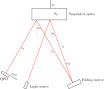
\includegraphics[width=104mm]{figures/folded_optical_lever}
	\caption{A schematic of the folded optical lever setup in KAGRA.}
	\label{fig:foldedopticallever}
\end{figure}
Fig.~\ref{fig:foldedopticallever} shows a folded optical lever setup.
This is a rare setup used for some optics, whose chamber doesn't have a viewport for the beam to exit after the first reflection.
In this configuration, the light beam hits the optics with an incidence angle of $\alpha_1$, and travels some distances $r_1$ towards a folding mirror inside the chamber.
The beam then hits the folding mirror with an incidence angle of $\alpha_2$, and travels along $r_2$ back to the optics.
At last, the beam hits the optics again with a difference angle of incidneces $\alpha_3$, and then travels $r_3$ to reach the QPD, which measures the beam spot displacement $x_\mathrm{tilt}$.

\begin{figure}[!h]
	\centering
	
\includegraphics[width=181mm]{figures/folded_optical_lever_rtm}
	\caption{A yaw of the optics can be treated as three path segments $r_1$, $r_2$, and $r_3$ in a folded optical lever configuration.}
	\label{fig:foldedopticalleverrtm}
\end{figure}
Let's consider an angular displacement in yaw, as shown in Fig.~\ref{fig:foldedopticalleverrtm}.
Black line formed by $r_1$, $r_2$, and $r_3$ is the original path of the beam.
As can be inferred from Eqn.~\eqref{eqn:x1}, a rotation of the optics, say by an amount $\theta_Y$ is equivalent to adding an angle $2\theta_Y$ to the beam path.
Hence, the angles of the path $r_1$ and $r_2$ are $2\theta_Y$, and that of $r_3$ is $2\theta_Y + 2\theta_Y=4\theta_Y$ (reflected twice).
So, the displacement of the beam spot at the QPD plane can be straightforwardly derived via the ray transfer matrix,
\begin{equation}
	\begin{pmatrix}
		x_\mathrm{tilt}\\
		\cdot
	\end{pmatrix}
	=
	\begin{bmatrix}
		1 & r_1+r_2\\
		0 & 1
	\end{bmatrix}
	\begin{pmatrix}
		0\\
		2\theta_Y
	\end{pmatrix}
	+
	\begin{bmatrix}
		1 & r_3\\
		0 & 1
	\end{bmatrix}
	\begin{pmatrix}
		0\\
		4\theta_Y
	\end{pmatrix},
\end{equation}
which gives
\begin{equation}
	x_\mathrm{tilt} = \left(2r_1+2r_2+4r_3\right)\theta_Y.
\end{equation}

Now, let's consider a longitudinal shift of the optics.
Similar to that of a regular optical lever, a longituidnal displacement is going to introduce a beam shift of $\left(2\sin\alpha_1\right)x_L$ at the first reflection.
A second beam shift of $\left(-2\sin\alpha_3\right)x_L$ is introduced in the return path to the QPD.
This gives a total beam spot displacement of $2\left(\sin\alpha_1-\sin\alpha_3\right)x_L$ at the QPD plane.
Without loss of generality, let's write down the beam spot displacement due to a rotation in yaw and a longitudinal shift,
\begin{equation}
	x_\mathrm{tilt} = \left(2r_1+2r_2+4r_3\right)\theta_Y + 2\left(\sin\alpha_1-\sin\alpha_3\right)x_L.
	\label{eqn:x_tilt_folded}
\end{equation}
Comparing Eqn.~\eqref{eqn:beam_displacement_l} and Eqn.~\eqref{eqn:x_tilt_folded}, we see that the effective arm length of yaw is 4 times that of a regular optical lever, if we assume $r_1=r_2=r_3=r$.
Also, if the incidence angles $\alpha_1$ and $\alpha_3$ are exactly the same, then the QPD readout will be completely decoupled from longituindal displacement of the optics.
However, this cannot be true if we consider a configuration as shown in Fig.~\ref{fig:foldedopticallever}.
The angle of incidence $\alpha_3$ is related to the other angle of incidences by
\begin{equation}
	\alpha_3 = \alpha_1+2\alpha_2.
\end{equation}
Having equal $\alpha_1$ and $\alpha_3$ would necessarily implies that $\alpha_2=0$.
This means that the beam goes back to via the same path and returns to the light source, which is physically impossible.
Therefore, there exists this irremovable longitudinal-to-yaw coupling.
Not to mention, the cross-coupling due to miscentered beam, as discussed in Sec.~\ref{sec:miscentered_beam_spot}, still exist and is also irremovable.

\subsubsection{Augmented folded optical lever}
\begin{figure}[!h]
	\centering
	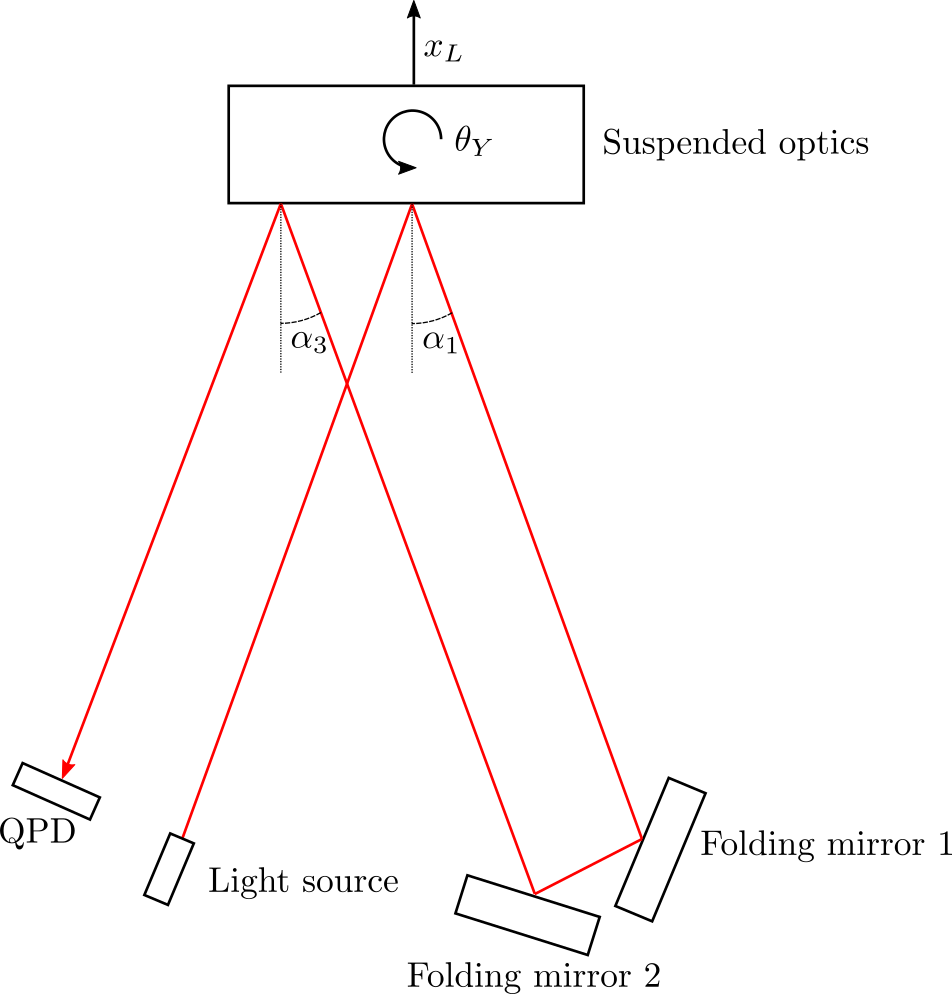
\includegraphics[width=81mm]{figures/folded_optical_lever_augmented}
	\caption{Folded optical lever augmented by adding a second folding mirror.}
	\label{fig:foldedopticalleveraugmented}
\end{figure}
As is discussed in the Sec.~\ref{sec:folded_optical_lever}, the QPD will sense both yaw and longitudinal displacement due to asymmetric angle of incidences between the forward and return path.
Here, as shown in Fig.~\ref{fig:foldedopticalleveraugmented}, we propose an augmented configuration where a second folding mirror is added.
In this configuration, the we can finely tweak the orientation of the second folding mirror to equalize the angle of incidences $\alpha_1$ and $\alpha_3$.
This way we can minimize the longitudinal coupling due to difference in angle of incidences.
However, this cannot fix the problem as discussed in Sec.~\ref{sec:miscentered_beam_spot}, so there will be residual uncertain coupling due to a miscentered beam.
%We would normally estimate the coupling ratio by measuring $\frac{x_\mathrm{len}'}{\theta_Y}$ at the yaw resonance frequency\footnote{We can estimate the yaw displacement using the tilt-sensing QPD. This is only valid at pure resonance and when there's no external line excitation.}.
%However, we have two unknowns here, namely $\delta_x$ and $\delta_d$.
%So, we cannot estimate the misplacement of the length-sensing QPD and the miscentering of the beam spot.




